%%%-------------------------------------------------------------------------
%%% PD3プレゼンプレート
%%% 作成: 金沢工大・情報工学科・鷹合研究室
%%%-------------------------------------------------------------------------

%
% このファイルは書き換えないで下さい
%
\documentclass[25pt, landscape,dvipdfmx, oneside, uplatex]{foils}

% 4:3のスクリーン(8号館)
\usepackage[top=15truemm,bottom=22truemm,left=15truemm,right=15truemm,paperwidth=300truemm,paperheight=225truemm]{geometry}

% 16:9のスクリーン(23号館)
%\usepackage[top=15truemm,bottom=22truemm,left=15truemm,right=15truemm,paperwidth=320truemm,paperheight=180truemm]{geometry}
\setlength{\foilheadskip}{0mm}
\setlength{\parindent}{0mm}

\usepackage[deluxe,uplatex]{otf}
\usepackage[T1]{fontenc}
\usepackage{lmodern}
\renewcommand{\kanjifamilydefault}{\gtdefault}  % 日本語フォントをゴシックに
\mathversion{bold} % 数式フォントを太字に変更する


\usepackage{bbding} % \PencilRightDown 鉛筆マーク
\usepackage{tikz}
\usepackage[symbol]{footmisc}
\usepackage{xcolor,listings, plistings}
\usepackage{multicol}
\usepackage{url}
\usepackage{graphicx}
\usepackage{epsfig}

\usepackage{enumerate}
\usepackage{lastpage}
\usepackage{ascmac}
\usepackage{fancybox,fancyvrb,okumacro}

\renewcommand{\lstlistingname}{List} 
\usepackage[%
pdfstartview={FitH -32768},%    描画領域の幅に合わせる
bookmarks=true,%                しおり付き
bookmarksnumbered=true,%        章や節の番号をふる
bookmarkstype=toc,%             目次情報のファイル.tocを参照
colorlinks=true,%              ハイパーリンクを色枠に
linkcolor=black,%
urlcolor=black,%
citecolor=black,%
filecolor=black,%
menucolor=black,%
pagecolor=black,%
]{hyperref}
\lstset{%
	language={Python}, 
	backgroundcolor={\color[gray]{.95}},%
	basicstyle={\ttfamily\small},%
	identifierstyle={\ttfamily\small},
	commentstyle={\ttfamily\small\color{red}},
	keywordstyle={\ttfamily\small\color{blue}},
	ndkeywordstyle={},%
	stringstyle={\ttfamily\small\color[rgb]{0,0.5,0}},
	frame={tb},
	breaklines=true,
    columns=[l]{fullflexible},
%	columns=[l]{fixed},% fixed だと開きすぎ
	basewidth=0.5em,   % これないと行頭のスペースが揃わない
	numbers=left,%
	xrightmargin=0zw,%
	xleftmargin=3zw,%
	numberstyle={\ttfamily\small},%
	tabsize=3,
	stepnumber=1, 
	numbersep=0.75zw,%
	lineskip=-0.3ex,%
	belowcaptionskip=3pt,   % これないと見出しとリスト本体に隙間が毎回変わる
	abovecaptionskip=0pt,
	captionpos=t,
	showstringspaces=false, % 半角スペースを記号で表示しない
}
%

%%%%%%%%%%%% fboxの線幅
\setlength{\fboxrule}{1.5pt}



%%%%%%%%%%%% ページフッタの設定 %%%%%%%%%%%%%
\usepackage{fancyhdr}
\pagestyle{fancy}
\fancyhf{}  % これを入れないと2ページのフッタがずれる
\renewcommand{\headrulewidth}{0pt} % 水平線を消去
\renewcommand{\footrulewidth}{0pt} % 水平線を消去
\renewcommand{\thefootnote}{\fnsymbol{footnote}}


%%%%%%%%%%%%%%%%%%%%%%%%%%%%%%%%%%%%%%%%%
% 
% トップスライドのロゴ画像の設定 
%
%%%%%%%%%%%%%%%%%%%%%%%%%%%%%%%%%%%%%%%%%
\MyLogo{}
%% \MyLogo{\includegraphics[height=1.1cm]{fig/logo/kit_landscape1.eps}}

%%%%%%%%%%%%%%%%%%%%%%%%%%%%%%%%%%%%%%%%%
% 
% フッタ−の設定 
%
%%%%%%%%%%%%%%%%%%%%%%%%%%%%%%%%%%%%%%%%%

\lfoot{\small 鷹合研}
%\lfoot{\includegraphics[height=.75cm]{fig/logo/kit_landscape1.eps}} % 各スライドのロゴ画像
% NOTE:KITのロゴ画像の入手方法
%   http://mercury.kanazawa-it.ac.jp/koho/kitlogo/

\cfoot{\thepage/\pageref{LastPage}}
\rfoot{\small EPX-999} % テーマ番号

%%%%%%%%%%%%%%%%%%%%%%%%%%%%%%%%%%%%%%%%%
% 
% ここから下を書き換えて下さい 
%
%%%%%%%%%%%%%%%%%%%%%%%%%%%%%%%%%%%%%%%%%

\title{
{\large (12月 PD3進捗状況報告)}\\\vspace{10mm}
{\LARGE PDⅢ活動における\\「やるやる詐欺」の傾向と対策}
}
\date{情報工学科 鷹合研究室}
\author{
3EP5-05\\ \ruby{織田}{おだ}\ruby{信秀}{のぶひで} \and
3EP5-15\\ \ruby{織田}{おだ}\ruby{信長}{のぶなが} \and 
3EP5-22\\ \ruby{織田}{おだ}\ruby{信雄}{のぶかつ}
}



\begin{document}
\maketitle % タイトルページ

%%%%%%%%%%%%%%%%%%%%%%%%%%%%%
\foilhead[-14mm]{\Large 1. はじめに -- 背景と目的 -- }
\begin{itemize} 
%\setlength{\itemsep}{-0.2cm} % 項目間の行間を詰めたい時に指定して下さい
 \item 現在,何が問題か(あるいは将来,何が問題になるか)を書く.
 \item その問題に対処するためには,どのようなものがあればよいか(あるいは取り組みが必要)かを書く.
 \item 本プロジェクトでは何を使ってどんなものを作っているかを書く.
\end{itemize}
\newpage

%%%%%%%%%%%%%%%%%%%%%%%%%%%%%
\foilhead[-14mm]{\Large 発表の流れ}
\begin{enumerate}
	\item {\color{gray}はじめに -- 背景と目的 --}
	\item システム概要
	\item 評価
	\item むすび
\end{enumerate}
\newpage

%%%%%%%%%%%%%%%%%%%%%%%%%%%%%%%%%%%%%%%%%%%%%%
\foilhead[-14mm]{\Large 2. システム概要}

ここにブロック図をいれシステム全体を解説する.ドローンや車両などを開発した場合は,その写真も示す.
\begin{figure}[h]
\begin{center}
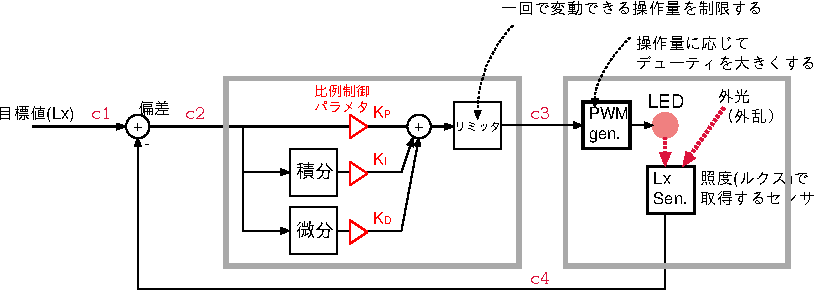
\includegraphics[width=\textwidth]{fig/system.pdf}
\caption{あああああああ}
\end{center}
\end{figure}
\newpage

%%%%%%%%%%%%%%%%%%%%%%%%%%%%%%%%%%%%%%%%%%%%%%
\foilhead[-14mm]{\Large 2-1. 畳み込みニューラルネットワークの構造}
\begin{description} 
	\item[①入力層]~\\
	ああああああああああああああああああああああいいいいいいいいいいいいいいいいいいいいいいいいいいいいいいいいいいいいいいいうううううううううううううううう
	\item[②中間層]~\\
	ああああああああああああああああああああああいいいいいいいいいいいいいいいいいいいいいいいいいいいいいいいいいいいいいいいうううううううううううううううう
	\item[③出力層]~\\
	ああああああああああああああああああああああいいいいいいいいいいいいいいいいいいいいいいいいいいいいいいいいいいいいいいいうううううううううううううううう
\end{description}
\newpage

%%%%%%%%%%%%%%%%%%%%%%%%%%%%%%%%%%%%%%%%%%%%%%
\foilhead[-14mm]{\Large 2-2. ○○○○○処理の方法}
\begin{description} 
	\item[①Javascript]~\\
	ああああああああああああああああああああああいいいいいいいいいいいいいいいいいいいいいいいいいいいいいいいいいいいいいいいうううううううううううううううう
	\item[②Python+Tornado]~\\
	ああああああああああああああああああああああいいいいいいいいいいいいいいいいいいいいいいいいいいいいいいいいいいいいいいいうううううううううううううううう
	\item[③pigpio]~\\
	ああああああああああああああああああああああいいいいいいいいいいいいいいいいいいいいいいいいいいいいいいいいいいいいいいいうううううううううううううううう
\end{description}
\newpage


%%%%%%%%%%%%%%%%%%%%%%%%%%%%%%%%%%%%%%%%%%%%%%
\foilhead[-14mm]{\Large 3. 評価・考察}
\begin{itemize}
	\item このスライドでは何をどのような方法で評価したかを明記し,結果をグラフで示すこと(表よりグラフのほうが良い).
	\item システムが動いている様子がわかるようにデモ映像を流すこと(デモ映像には字幕をつけたりするなどしてわかりやすくすること).
	\item 評価の際は,改良の前後でどうなったかを示す.あるいは他の手法などと比較してどうなのかを示すことも必要.
	\item 結果について考察も示すこと.
\end{itemize}
\newpage

%%%%%%%%%%%%%%%%%%%%%%%%%%%%%%%%%%%%%%%%%%%%%%
\foilhead[-14mm]{\Large 4. むすび}
\begin{itemize}
	\item 何のために何を作成したかを改めて書く.
	\item 現時点での評価結果,考察を簡潔に書く.
	\item 来月の報告までに何をするか計画を書く.
\end{itemize}
\newpage

%%%%%%%%%%%%%%%%%%%%%%%%%%%%%%%%%%%%%
ここからおまけ
\lstinputlisting[language=c, caption=test2.c]{src/hello.c}
\lstinputlisting[language=python, caption=test2.py]{src/world.py}


\end{document} 
